    \section{Część praktyczna}
    \subsection{Dyskretny problem plecakowy}
    \subsubsection{Rozwiązanie wyczerpujące}
    
    Przegląd wyczerpujący wymaga przeszukania całego zbioru rozwiązań i znalezienia w ten sposób rozwiązania optymalnego. Zbiór rozwiązań jest zbiorem wszystkich podbiorów zbioru elementów, z których wybieramy te, które mają się znaleźć w plecaku. W związku z tym, takich podzbiorów jest $2^n$, gdzie $n$ to liczba elementów, z których wybieramy.
    
    \subsubsection{Wartości funkcji oceny}
    
    Celem pierwszego eksperymentu było zbadanie parametrów rozwiązania uzyskanych za pomocą heurystyki i porównanie ich z metodą przeglądu wyczerpującego. Za pomocą liczb pseudolosowych wybrano wartości oraz masy przedmiotów dla zadanej ich liczby. Maksymalna masa plecaka, w każdym powtórzeniu programu wynosiła połowę sumy mas wszystkich wylosowanych przedmiotów. Zakres mas przedmiotów oraz ich wartości zawierały się w zadanym przedziale i miały wartości całkowite. Z uwagi na fakt, że eksperyment uwzględniał użycie liczb pseudolosowych, Był on powtarzany wielokrotnie.
    
    W tabeli przedstawione zostały rezultaty badań dla różnych przedziałów wartości i mas przedmiotów dla stałej liczby przedmiotów.
    
    \begin{table}[h!]
    	\centering
    	\begin{tabular}{ |p{4cm}||p{2cm}|p{2cm}|p{2cm}|p{2cm}|p{2cm}| }
    		
    		\hline
    		\multicolumn{5}{|c|}{Parametry rozwiązania za pomocą heurystyki w porównaniu do przeglądu wyczerpującego} \\
    		\hline
    		liczba iteracji & 25 & 25 & 25 & 25 \\
    		\hline
    		liczba elementów & 12 & 12 & 25 & 12 \\
    		\hline
        	Zakres wartości przedmiotów i mas & (1, 10) & (1, 100) & (90,100) & (900, 1000) \\
    		\hline
    		współczynnik rozwiązań optymalnych & 0.73 & 0.71 & 0.12 & 0.17 \\
    		\hline
    		maksymalny błąd bezwzględny & 4 & 32 & 10 & 119 \\
    		\hline
    		maksymalny błąd względny & 0.09 & 0.07 & 0.02 & 0.02 \\
    		\hline
    		średnia wartość błędu bezwględnego & 0.46 & 4.19 & 3.78 & 35.97 \\
    		\hline
    		średnia wartość błędu względnego & 0.01 & 0.01 & 0.01 & 0.01 \\
    		\hline
    		odchylenie standardowe błędu bezwzględnego & 0.93 & 7.82 & 2.57 & 31.21 \\
    		\hline
    		odchylenie standardowe błędu bezwzględnego & 0.02 & 0.02 & 0.01 & 0.01 \\
    		\hline
    	\end{tabular}
    	\caption{Rezultaty pomiarów}
    \end{table}
	Z pomiarów wynika, że pomimo tego że, wraz ze wzrostem zakresu wartości i mas przedmiotów maleje współczynnik rozwiązań optymalnych osiąganych przez algorytm heurystyczny. Pomimo jednak, że wzrasta również średnia wartość błędu bezwględnego, w tym samym czasie wartość średniego błędu względnego i maksymalnego błędu średniego są stosunkowo małe - Stanowią zaledwie kilka procent wartości optymalnej. 
    \subsubsection{Czas działania programu}
    W miarę wzrostu liczby przedmiotów zwiększa się liczba możliwych rozwiązań, a więc i czas wyznaczenia rozwiązania. Celem drugiego eksperymentu było zbadanie, w jaki sposób rośnie ta zależność. Mierzony był czas działania programu. Z uwagi na to, że liczba operacji jest niemal taka sama niezależnie od parametrów przedmiotów, dla jednej ich liczby był wykonowany tylko jeden pomiar, w celu redukcji trwania ekperymentu. Proces był powtarzany tak długo, aż czas działania solwera optymalnego wyniósł więcej niż 1 minuta. Ten sam test, dla tych samych zmiennych był wykonywany dla obu solwerów.
    
    
    Na wykresach przedstawiono zależność czasu działania programu od liczby przedmiotów dla obu solwerów w skalach liniowej oraz logarytmicznej.
    
    
	\begin{figure}[h!]
		\centering
		\begin{subfigure}[b]{0.45\linewidth}
			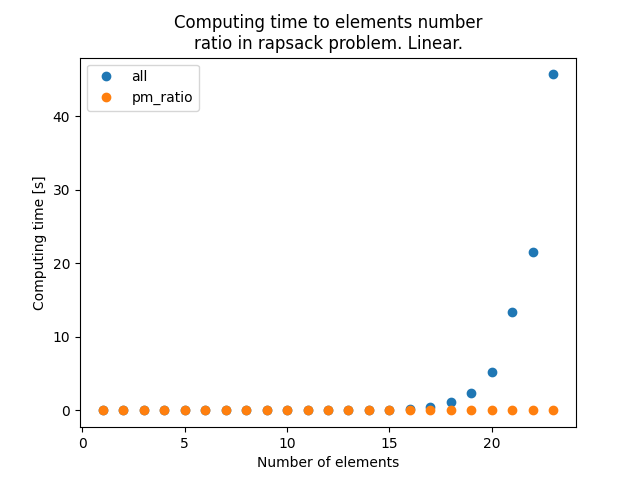
\includegraphics[width=\linewidth]{photos/test_lin.png}
			\caption{Skala liniowa}
		\end{subfigure}
		\begin{subfigure}[b]{0.45\linewidth}
			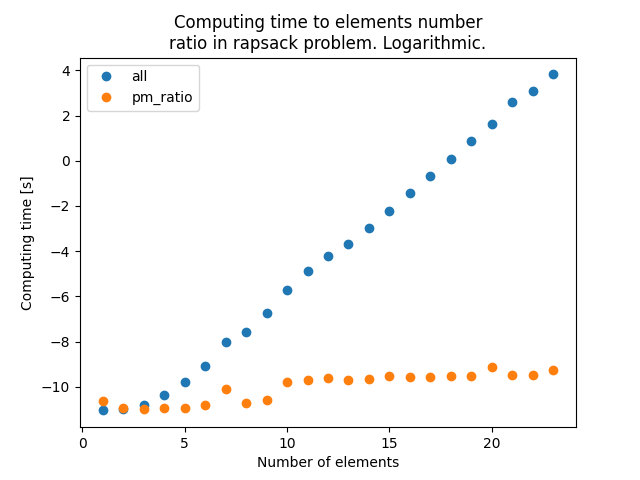
\includegraphics[width=\linewidth]{photos/test_log.png}
			\caption{Skala logarytmiczna}
		\end{subfigure}
		\caption{Wykresy zależności czasu obliczeń od liczby przedmiotów}
	\end{figure}
	
    Pomiar czasu wyższy niż 60 sekund zaobserwowano dla $n=23$.

	Warto zauważyć, że wyniki przyjmują postać liniową w skali logarytmiczej, co sugeruje, że w skali liniowej wraz ze wzrostem liczby elementów czas obliczeń rośnie wykładniczo. Dla 22 przedmiotów plecaku czas obliczeń wyniósł ok. 42 sekundy, natomiast po dodaniu jednego przedmiotu Czas wyniósł ponad 80 sekund, czyli ok. dwukrotnie więcej niż dla 22 sekund. Zgadza się to z teoretyczną złożonością.	

    
    \subsection{Metoda najszybszego wzrostu}

	\subsubsection{Wpływ współczynnika $\beta$}
	Współczynnik $\beta$ wpływa na to, o jakiej długości krok przesunie się obecnie badany punkt. Jego wartość ma zatem kluczowy wpływ na zachowanie algorytmu.
	Wartości współczynnika $\beta$ użyte w trakcie powyższego eksperymentu zostały wyznaczone w taki sposób, aby dla punku startowego przy uwzględnieniu ograniczeń kostkowych, działanie algorytmu było zbieżne. Ciekawym się okazało, to, że po pewnej liczbie iteracji, można zmniejszyć wartość współczynnika nawet o kilka rzędów wielkości, a działanie algorytmu dalej będzie zbieżne.

	\subsubsection{Zachowanie algorytmu}
	W celu zobaczenia zachowywania się algorytmu zostały zrobione generatory wykresów przedstawiające kolejne kroki algorytmu na tle poziomic. Dla każdej z badanych funkcji zostały otworzone 3 różne wykresy dla różnych punktów startowych dla zadanej funkcji. Funkcja booth jest funkcją, która przyjmuje wektory o wymiarze równym 2. Funkcje CEC2017 natomiast przyjmują jako argumenty wektory o wymiarze równym 10. W związku z tym, dla każdej funkcji wykres został utworzony trzykrotnie dla różnych kombinacji wymiarów przedstawianych. Założono, że podczas generowania poziomic, wartości argumentów, których wymiar nie jest badanych, mają wartości równe 0. 
	\begin{itemize}
		\item Funkcja booth
		 \begin{itemize}
		 	\item Funkcja booth była stosunkową dobrze uwarunkowaną funkcją i już po kilkudziesięciu iteracjach algorytmu uzyskiwało się przyzwoity wynik.
		 	\item Minimum funkcji jest w punkcie $x = (1, 3)$ i wynosi $f(x) = 0$.
		 \end{itemize}
		\item CEC2017 f1
		\begin{itemize}
			\item Funkcja CEC2017 f1 była najlepiej uwarunkowaną funkcją z testowanych funkcji z grupy CEC2017. Stosunkowo szybko zbiegała do minimum. Wartość współczynnika $\beta$, dla którego funkcja zbiegała z niemal każdego punku wyniosła ~$10^{-8}$.
			\item Minimum funkcji jest w punkcie:
			    \begin{lstlisting}[language=Python]
x = [
	-49.24189985,
	-70.42955972,
	-29.61018187,
	-58.32676328,
	22.08960188,
	59.93874989,
	36.76670148,
	18.55873627,
	76.68042093,
	-37.25371714
]
				\end{lstlisting}
			i wynosi $f(x) = 200.7140013364138$.
		\end{itemize}
	\item CEC2017 f2 oraz f3
	\begin{itemize}
		\item Funkcje CEC2017 f2 i f3 oraz ich gradienty przyjmują bardzo duże wartości. W związku z tym Potrzebne są w ich przypadku bardzo małe wartości współczynnika $\beta$. Przy stałym współczynniku, funkcje coraz wolniej zbiegają do swojego minimum i dojście do celu jest bardzo czasochłonne i kosztowne. Jak widać na rysunkach, pomimo dużej liczby iteracji oprogramowania, droga widoczna na wykresach jest stosunkowo krótka w porównaniu do wcześniej badanych funkcji. Widoczna jest tutaj główna wada algorytmu - brak zmiennego kroku, który pozwoliłby funcji na podtrzymywanie tempa docierania do minimum.
			\item Minimum funkcji f2 jest w punkcie:
\begin{lstlisting}[language=Python]
x = [
	-29.31995891,
	-16.76540101,
	-75.46834234,
	-0.63716325,
	4.30364919,
	-37.55999386,
	42.94548049,
	74.7345723,
	-63.04848011,
	71.32898298,
]
\end{lstlisting}
			i wynosi $f(x) = 200.0295524387396$.
			\item Minimum funkcji f3 jest w punkcie:
\begin{lstlisting}[language=Python]
x = [
	-56.00495921,
	4.49247818,
	35.32391443,
	8.23436017,
	-47.24491346,
	7.29982139,
	6.42709164,
	-2.54886095,
	-61.00295813,
	-47.12330431
]
\end{lstlisting}
i wynosi $f(x) = 300.0533132041394$.
	\end{itemize}
	\end{itemize}


